\documentclass[12pt]{article}

\usepackage{sbc-template}
\usepackage{graphicx,url}
\usepackage{float}
\usepackage{array}
\usepackage[brazilian]{babel}
\usepackage[utf8]{inputenc}
\usepackage[T1]{fontenc}
\usepackage{placeins}
\usepackage{tablefootnote} 
\raggedbottom 
\floatstyle{plaintop}
\newfloat{quadro}{htbp}{loq}
\floatname{quadro}{Quadro}
\usepackage{booktabs}

\sloppy

\title{BeatleXML - Automação de Processos Fiscais: O Impacto da Tecnologia no Compliance Contábil}

\author{Wilian Fragata dos Santos\inst{1}, Claudia Bocchese de Lima\inst{1}, \\ Eduardo Luiz Alba\inst{1}}

\address{
Instituto Federal do Paraná (IFPR) -- Campus Palmas\\
Bacharelado em Sistemas de Informação\\
Palmas -- PR -- Brasil
\email{\{william\_fragatta\}@hotmail.com}
\email{\{claudia.bocchese, eduardo.alba\}@ifpr.edu.br}
}

\begin{document}

\maketitle

% ================= abstract e resumo =================

\begin{abstract}
This work presents the development of the BeatleXML system, a secure web platform built to automate the capture and organization of electronic tax documents: the Electronic Tax Invoice (NF-e), and the Electronic Consumer Tax Invoice (NFC-e). Aimed at solving communication challenges between companies and accounting firms, the platform acts as a digital bridge, centralizing tax files in a cloud repository. The solution eliminates the manual collection of documents, enables real-time purchase auditing, and provides financial organization tools for companies. Simultaneously, it offers accountants a dashboard for bulk downloads, which is essential for monthly accounting closings. From a Software Engineering perspective, the project details the use of background workers to consume government Application Programming Interfaces (APIs), as well as the creation of autonomous desktop agents for monitoring local directories. Additionally, the system consolidates the application of privacy principles in compliance with the Brazilian General Data Protection Law (LGPD). This is achieved through the architectural isolation of client data (\textit{multi-tenant}), Role-Based Access Control (RBAC), and the use of symmetric cryptography to protect digital certificates.

\textbf{Keywords:} Process automation; Accounting compliance; Electronic tax documents; Systems integration; Privacy by Design.
\end{abstract}

\begin{resumo} 
Este trabalho apresenta o desenvolvimento do sistema BeatleXML, uma plataforma web segura construída para automatizar a captura e a organização de documentos fiscais eletrônicos: a Nota Fiscal Eletrônica (NF-e) e a Nota Fiscal de Consumidor Eletrônica (NFC-e). Direcionada a solucionar as dificuldades de comunicação entre empresas e escritórios de contabilidade, a plataforma atua como uma ponte digital, centralizando arquivos fiscais em um repositório em nuvem. A solução elimina a cobrança manual de documentos, viabiliza a auditoria de compras em tempo real e fornece ferramentas de organização financeira para as empresas. Simultaneamente, oferece aos contadores um painel para \textit{downloads} em lote, essencial para os fechamentos contábeis. Sob a ótica da Engenharia de Software, o projeto detalha o uso de rotinas em segundo plano (\textit{background workers}) para o consumo de Interfaces de Programação de Aplicações (APIs) governamentais, além da criação de agentes locais autônomos (\textit{desktop}) para o monitoramento de diretórios físicos. Adicionalmente, o sistema consolida a aplicação de princípios de privacidade em conformidade com a Lei Geral de Proteção de Dados (LGPD). Isso é alcançado por meio do isolamento arquitetural de dados entre clientes (\textit{multi-tenant}), do Controle de Acesso Baseado em Papéis (RBAC - \textit{Role-Based Access Control}) e do emprego de criptografia simétrica para a proteção de certificados digitais.

\textbf{Palavras-chave:} Automação de processos; Compliance contábil; Documentos fiscais eletrônicos; Integração de sistemas; Segurança da Informação.
\end{resumo}

% ================= Introdução =================

\section{Introdução}

A contabilidade moderna e a gestão empresarial dependem da troca rápida e segura de informações para o suporte estratégico à tomada de decisões \cite{laudon2014}. Com a digitalização dos processos fiscais no Brasil e a consolidação do Sistema Público de Escrituração Digital (SPED), os documentos físicos foram substituídos por arquivos digitais estruturados, exigindo drásticas adaptações sistêmicas por parte das organizações comerciais \cite{marion2020}. Nesse cenário, um dos principais desafios enfrentados por escritórios de contabilidade é a coleta mensal e tempestiva desses documentos eletrônicos para o fechamento contábil e fiscal \cite{castro2025}.

As empresas utilizam diferentes plataformas de gestão integrada, conhecidas como ERPs (\textit{Enterprise Resource Planning}), cada uma operando com lógicas distintas de armazenamento. Arquivos no formato \textit{Extensible Markup Language} (XML), gerados diariamente nos caixas de supermercados e comércios (os cupons fiscais, ou NFC-e), frequentemente ficam dispersos em computadores locais. Consequentemente, o ato de reunir e enviar essas informações ao contador torna-se um processo dependente de intervenção humana, sujeito a falhas, extravios e atrasos que comprometem prazos governamentais e sujeitam as entidades a pesadas multas \cite{tavares2018}.

Simultaneamente, existe o desafio da captação das Notas Fiscais Eletrônicas (NF-e) emitidas por fornecedores contra o Cadastro Nacional da Pessoa Jurídica (CNPJ) da empresa. Para obter esses dados de forma automatizada, é necessário consumir as interfaces de programação (APIs) disponibilizadas pelos Web Services da Secretaria de Estado da Fazenda (SEFAZ).

% ================= Objetivos  =================

\subsection{Objetivo Geral}

O objetivo geral desta pesquisa é desenvolver o BeatleXML, uma plataforma web segura e autônoma para atuar como uma "ponte digital" entre as rotinas da gestão empresarial e os escritórios de contabilidade. 

\subsection{Objetivos Específicos}

Para viabilizar este escopo, a pesquisa fundamentou-se em prover soluções humanas e organizacionais através da tecnologia, definindo os seguintes objetivos específicos:
\begin{itemize}
    \item Ajudar escritórios de contabilidade a acessar de forma instantânea e simultânea os documentos fiscais de todos os seus clientes, permitindo a baixa em lote (arquivos ZIP) sem a necessidade de cobrança manual via e-mail ou telefone;
    \item Prover aos gestores corporativos um painel que audite compras e centralize dados financeiros, reutilizando as informações de pagamento contidas nas notas fiscais para evitar juros por perda ou esquecimento de boletos;
    \item Capturar automaticamente as notas emitidas nos caixas físicos da empresa (NFC-e) através de um agente de software passivo instalado nos computadores locais, transferindo os dados para a nuvem em tempo real;
    \item Assegurar um tráfego de dados protegido e em total conformidade com a Lei Geral de Proteção de Dados (LGPD), garantindo a criptografia de senhas, a custódia segura de certificados digitais e controles rigorosos de acesso.
\end{itemize}

% ================= Justificativas  =================

\subsection{Justificativa e Contribuições}

A relevância deste trabalho justifica-se pela latente necessidade de eficiência operacional e mitigação de riscos legais \cite{laudon2014}. Do ponto de vista negocial, o sistema transforma o contador, que tradicionalmente atua como um "cobrador de arquivos", em um auditor proativo. Para as empresas, o sistema cessa o retrabalho de controle financeiro paralelo ao reaproveitar o arquivo fiscal XML, \textit{Extensible Markup Language}, gerado pelo governo para alimentar rotinas de contas a pagar.

Tecnologicamente, o projeto contribui ao demonstrar, na prática, a adoção de conceitos de Segurança desde a Concepção (\textit{Privacy by Design}). Ao implementar autenticação de dois fatores (2FA), controle de acessos hierárquicos e o mascaramento de dados sensíveis na base de dados, a plataforma resolve os problemas de interoperabilidade, \textit{compatibilidade entre sistemas}, e latência, \textit{tempo de atraso entre o envio de um arquivo, sinal ou comando e a chegada da resposta correspondente}, sem abrir mão do rigor exigido no tratamento de dados fiscais sigilosos.

% ================= REFERENCIAL TEÓRICO =================
\section{Referencial Teórico}

\subsection{O Impacto da Tecnologia na Contabilidade}
A evolução tecnológica transformou a contabilidade em uma ciência de dados voltada à tomada de decisão. Com a implementação do SPED, o Sistema Público de Escrituração Digital, o fisco brasileiro passou a exigir conformidade digital contínua das operações comerciais \cite{marion2020}. Nesse contexto, o \textit{compliance} contábil (a conformidade com as leis e regulamentos) tornou-se estritamente dependente da capacidade tecnológica das organizações. Sem o processamento ágil dos documentos, o profissional fica impossibilitado de concluir as escriturações nos prazos legais. Padoveze \cite{padoveze2015} destaca que sistemas de informações contábeis são fundamentais para garantir a sobrevivência financeira da empresa, mitigando riscos de autuações.

\subsection{Elicitação de Requisitos e Metodologias Ágeis}
Para que um \textit{software} corporativo seja aderente à realidade, é vital aplicar técnicas adequadas de elicitação de requisitos. Neste projeto, adotou-se o método de etnografia aplicado à Engenharia de Software \cite{sommerville2011}. A observação direta do fluxo de trabalho diário entre um supermercado e seu escritório de contabilidade evidenciou que a troca de documentos fiscais (especialmente notas de caixa) ocorria de forma manual, vulnerável e descentralizada. Os contadores dependiam de envios fragmentados por e-mail,  frequentemente com arquivos faltantes, ou através de aplicativos de mensagens instantâneas (como \textit{WhatsApp}), sem qualquer rastreabilidade ou segurança. Essa dor operacional inspirou diretamente a criação do agente autônomo \textit{Beatle Uploader}, suprimindo a intervenção humana no tráfego de dados.

A gestão do desenvolvimento baseou-se no paradigma das Metodologias Ágeis, combinando os \textit{frameworks} Scrum e Kanban \cite{pressman2016}. Essa abordagem permitiu iterações curtas e adaptação contínua às regras tributárias. O planejamento das tarefas e a estruturação visual das entregas foram conduzidos utilizando a plataforma de colaboração Miro, facilitando a documentação inicial e o refinamento da lógica.

\subsection{Arquitetura de Sistemas Web e Padrões de Comunicação}
O modelo estrutural adotado para o BeatleXML foi o de uma aplicação monolítica cliente-servidor organizada em três camadas (apresentação, negócio e dados) \cite{sommerville2011}. O paradigma monolítico foi escolhido pela eficiência em aplicações de escopo unificado, reduzindo a complexidade de manter múltiplos microsserviços para uma mesma regra de negócio. 

O modelo de comunicação obedece ao padrão de pedido-resposta (\textit{request-response}) síncrono e assíncrono sobre o protocolo HTTP (\textit{Hypertext Transfer Protocol}). Os programas locais (\textit{desktop}) atuam estritamente como clientes deste servidor web, enviando arquivos e consultando o estado do sistema, sem reter regras de negócio em suas bases.

\subsection{Stack Tecnológica e Segurança da Informação}
A escolha das tecnologias baseou-se na premissa de entregar um sistema rápido, mantendo a simplicidade operacional. A interface de usuário (\textit{frontend}) evitou a complexidade excessiva de aplicações de página única (SPAs). Adotou-se a renderização baseada em servidor (\textit{server-side rendering}) onde o motor de \textit{templates} Jinja2 processa o HTML diretamente. A estilização visual utilizou o \textit{framework} Tailwind CSS (via CDN) e ícones Font Awesome 6. A reatividade do painel e as requisições dinâmicas à API \textit{(Application Programming Interfaces)} utilizam JavaScript puro (\textit{Vanilla JS}), reduzindo a sobrecarga do navegador do cliente.

A camada de negócios (\textit{backend}) foi construída na linguagem Python (versão 3.11+). O núcleo de processamento é o \textit{framework} FastAPI, executado pelo servidor ASGI Uvicorn, escolhido por sua alta performance e suporte nativo a rotinas assíncronas \cite{pressman2016}. A integração com a SEFAZ \textit{(Secretaria de Estado da Fazenda)} demandou a leitura atenta do Manual de Orientação do Contribuinte (MOC), disponibilizado no Portal Nacional da NF-e. Contudo, a complexidade estrutural do modelo SOAP (\textit{Simple Object Access Protocol}) e a falta de clareza prática na documentação oficial forçaram o uso de técnicas de tentativa e erro e ambientes de homologação para estabilizar o consumo da API \textit{(Application Programming Interfaces)}. A comunicação final é gerenciada pelas bibliotecas \texttt{requests} e \texttt{requests-pkcs12}, enquanto a assinatura digital dos XMLs utiliza \texttt{signxml} e \texttt{lxml}.

Em consonância com a Lei Geral de Proteção de Dados (LGPD), a arquitetura incorpora a Segurança desde a Concepção (\textit{Privacy by Design}). A autenticação utiliza o padrão JWT (\textit{JSON Web Token}) gerado via \texttt{python-jose}. As senhas são protegidas por \textit{hashing} (\texttt{bcrypt}). O manuseio dos certificados digitais modelo A1 (\texttt{.pfx}) emprega criptografia simétrica com a biblioteca \texttt{cryptography} (\textit{Fernet}), e o acesso público é mitigado pelo serviço Google reCAPTCHA.

\subsection{Persistência e Estruturação de Dados}
O paradigma de banco de dados selecionado foi o Relacional (SQL). Em contraposição aos bancos Não-Relacionais (NoSQL, como MongoDB ou Firebase) — que organizam dados em documentos flexíveis —, o modelo relacional é imperativo para sistemas contábeis, que exigem estruturação tabular rígida, consistência transacional e relacionamentos fortemente tipados (chaves primárias e estrangeiras) \cite{laudon2014}. 

O Sistema Gerenciador de Banco de Dados (SGBD) escolhido foi o PostgreSQL. A integridade informacional é assegurada por restrições de unicidade (\textit{Unique Constraints}) nativas do banco, executadas dentro de transações de reversão automática (\textit{commit/rollback}). O acesso ao SGBD pela aplicação Python é abstraído pelo mapeador objeto-relacional (ORM) SQLAlchemy. O projeto também explora a flexibilidade híbrida do PostgreSQL, utilizando recursos como \textit{arrays} e objetos JSONB para o armazenamento pontual de estruturas dinâmicas, como as etiquetas customizadas pelo usuário.

\subsection{Trabalhos Correlatos e Soluções de Mercado}

Para avaliar o estado da prática, mapearam-se soluções comerciais disponíveis para a gestão documental fiscal. O Quadro \ref{qua:comparativo} apresenta uma síntese de quatro plataformas utilizadas no mercado, servindo de base para a distinção técnica do sistema proposto.

\begin{quadro}[H]
\centering
\scriptsize
\caption{Comparativo de Soluções de Mercado}
\vspace{0.2cm}
\begin{tabular}{p{2.5cm} p{3cm} p{4.5cm} p{4cm}}
\toprule
\textbf{Sistema} & \textbf{Foco Principal} & \textbf{Mecânica de Funcionamento} & \textbf{Diferencial do Projeto} \\ 
\midrule
\textbf{Sieg}\tablefootnote{\url{https://sieg.com}} & Escritórios de contabilidade. & Download automático de XMLs via certificado digital centralizado. & Arquitetura voltada simultaneamente para auditoria do gestor (varejo) e rotina contábil. \\ 
\textbf{Qive (Arquivei)}\tablefootnote{\url{https://qive.com.br}} & Captura e gestão de volumes em massa. & Consulta direta à SEFAZ \textit{(Secretaria de Estado da Fazenda)}, voltada para médias e grandes corporações. & Rotinas de \textit{background} e agente local autônomo (NFC-e). \\ 
\textbf{ContaAzul}\tablefootnote{\url{https://contaazul.com}} & ERP e Gestão Financeira PME. & Plataforma integrada com módulo de exportação contábil. & Arquitetura agnóstica; atua apenas como \textit{middleware} de arquivos. \\ 
\textbf{Nibo}\tablefootnote{\url{https://www.nibo.com.br}} & Portal de comunicação e gestão. & Gestão financeira com portal de upload de arquivos. & Elimina a dependência de \textit{upload} manual através de agente instalado. \\ 
\bottomrule
\end{tabular}
\vspace{0.1cm}
\centerline{\footnotesize Fonte: Elaborado pelo autor (2026).}
\label{qua:comparativo}
\end{quadro}

A análise estrutural dessas ferramentas indica que, embora eficientes em seus nichos, elas apresentam lacunas que o BeatleXML se propõe a preencher de forma unificada. Abaixo, detalham-se as principais diferenças metodológicas em relação a cada solução de mercado:

\begin{itemize}
    \item \textbf{Sieg:} Esta plataforma possui um excelente motor de captação, mas sua arquitetura é focada quase exclusivamente no fluxo de trabalho interno do contador. O BeatleXML diverge ao conceder total autonomia à empresa cliente, fornecendo a ela um painel próprio para auditar compras e organizar o fluxo financeiro de contas a pagar antes mesmo do contador agir.
    
    \item \textbf{Qive (Arquivei):} Voltada para grandes corporações e gestão de dados em massa (Big Data fiscal). O diferencial do BeatleXML encontra-se na sua acessibilidade para o pequeno e médio varejo e, de forma contundente, na solução do envio de cupons de frente de caixa (NFC-e), problema resolvido diretamente pelo agente de monitoramento (\textit{watchdog}) instalado na máquina do cliente.
    
    \item \textbf{ContaAzul:} Opera como um Sistema Integrado de Gestão Empresarial (ERP \textit{(Enterprise Resource Planning)}) completo. Para utilizá-lo na plenitude, o varejista precisa abandonar suas ferramentas atuais e adotar o ecossistema ContaAzul para faturamento e estoque. O BeatleXML é tecnicamente \textit{agnóstico}: ele não substitui o ERP \textit{(Enterprise Resource Planning)} legatário do cliente, operando silenciosamente nos bastidores como uma ponte de comunicação via leitura de diretórios.
    
    \item \textbf{Nibo:} Atua fortemente como um portal de comunicação entre a empresa e o contador. Contudo, a submissão de documentos locais exige que o operador humano acesse o portal, selecione as pastas e realize o \textit{upload}. O diferencial do projeto proposto é justamente a automação desse passo, eliminando o fator de esquecimento humano ao transferir essa responsabilidade para um serviço de sistema operacional invisível ao usuário.
\end{itemize}

% ================= METODOLOGIA E ARQUITETURA =================\section{Metodologia e Arquitetura do Sistema}

% ================= METODOLOGIA =================
\section{Metodologia}

Esta pesquisa caracteriza-se como um estudo aplicado e descritivo, voltado à documentação de um problema prático de gestão da informação e ao desenvolvimento de uma proposta tecnológica para auxiliá-lo. Para facilitar a compreensão do trabalho realizado, a metodologia foi organizada de forma cronológica, acompanhando desde a observação inicial do problema no ambiente de trabalho até o planejamento, construção e testes da plataforma web. As etapas que compõem o ciclo de execução deste estudo são apresentadas na Figura \ref{fig:metodologia}.

\begin{figure}[H]
\centering
\caption{Ciclo de Desenvolvimento do Projeto}
\vspace{0.2cm}
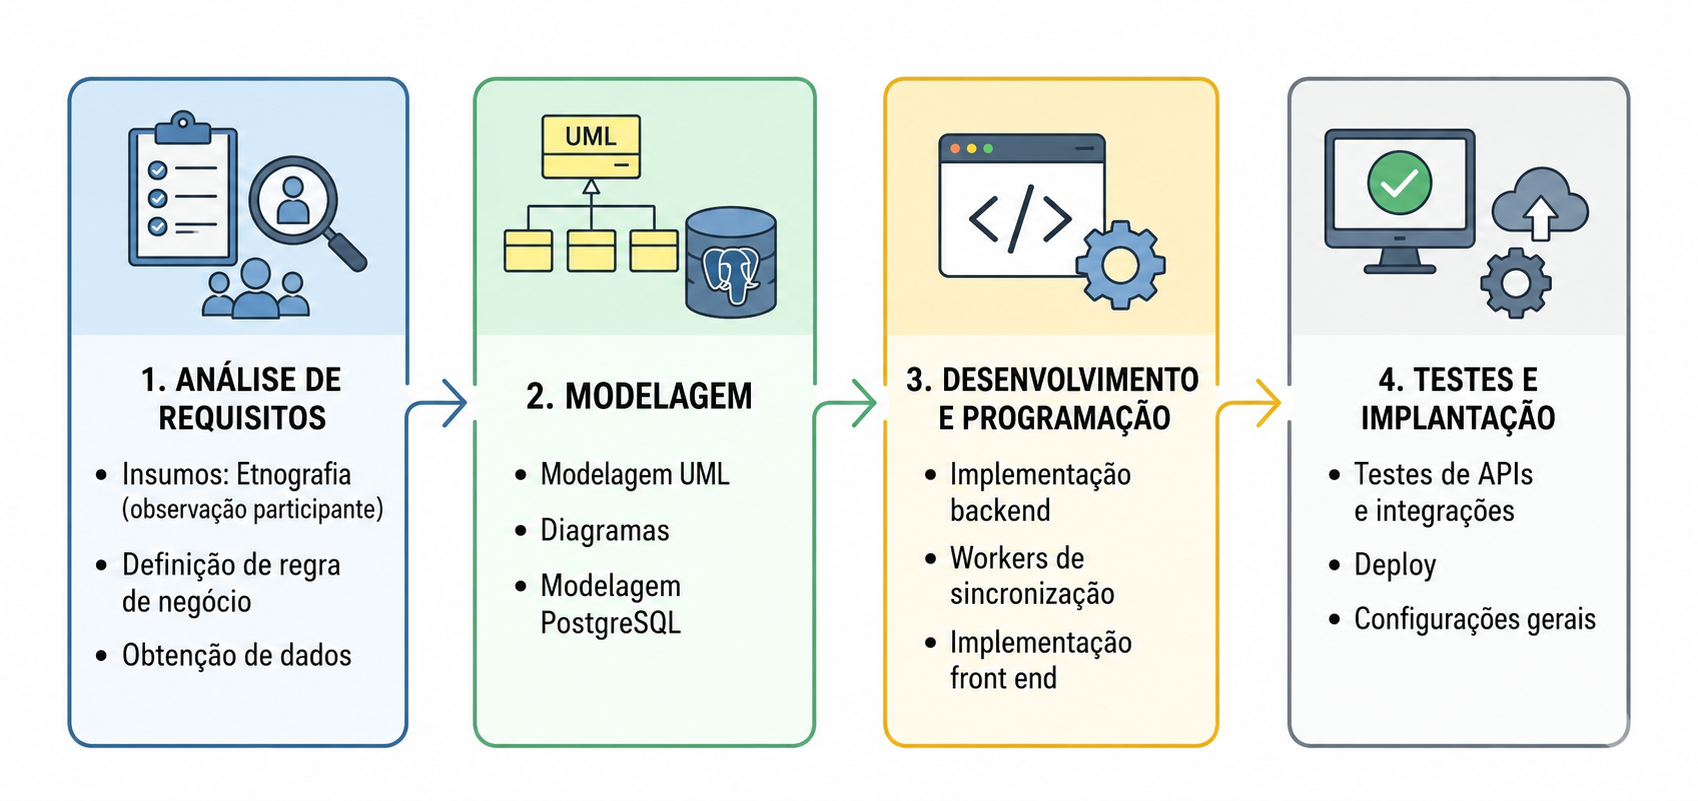
\includegraphics[width=0.9\textwidth]{metodologia.png}
\vspace{0.2cm}
\centerline{\footnotesize Fonte: Elaborado pelo autor (2026).}
\label{fig:metodologia}
\end{figure}

\subsection{Abordagem Etnográfica e Identificação do Problema}

Na Engenharia de Software, compreender a rotina real dos usuários antes de iniciar a programação é uma etapa essencial para evitar a criação de ferramentas desconectadas da prática. Para levantar as necessidades deste projeto, utilizou-se o método da etnografia por observação participante. Trata-se de uma abordagem de pesquisa qualitativa em que o pesquisador está inserido diretamente no cotidiano do grupo estudado, observando os processos, as dificuldades e a cultura de trabalho a partir da perspectiva de quem executa as tarefas diariamente \cite{sommerville2011}.

A escolha desse método justifica-se pela atuação direta do autor no setor administrativo e financeiro de um grupo empresarial varejista, aliada à formação acadêmica nas áreas de Sistemas de Informação e Ciências Contábeis. Essa vivência permitiu observar simultaneamente as necessidades tecnológicas e as exigências fiscais da rotina diária.

O ambiente observado é composto por três empresas do mesmo grupo econômico: dois supermercados (sendo uma matriz e uma filial) e uma loja do ramo de papelaria. Embora possuam cadastros jurídicos (CNPJs) distintos, toda a gestão financeira e a preparação de documentos contábeis dessas três unidades ocorrem de maneira centralizada em um único escritório interno. Por outro lado, a contabilidade oficial, responsável pela apuração de impostos e entrega de declarações ao governo, é realizada por um escritório contábil terceirizado, localizado em outro endereço físico.

Durante o acompanhamento diário das rotinas entre o setor interno do grupo empresarial e o escritório terceirizado, verificou-se que o elevado volume diário de compras e vendas gerava gargalos operacionais em ambas as pontas do processo.

\subsubsection{Problemas Observados no Ambiente Interno da Empresa}

No cotidiano dos dois supermercados e da papelaria, a chegada de mercadorias enviadas por fornecedores ocorre de forma contínua. O principal problema identificado nesse fluxo refere-se ao momento da conferência das Notas Fiscais Eletrônicas (NF-e) de compra:

\begingroup
\setlength{\parskip}{0pt}
\setlength{\parindent}{0pt}

\textbf{Atrasos no recebimento de mercadorias:} Como o sistema de gestão interno (ERP \textit{(Enterprise Resource Planning)}) utilizado pelas lojas não possuía comunicação direta com a base de dados da Receita Federal, os funcionários só tinham acesso aos dados da nota fiscal quando o caminhão estacionava para descarregar e entregava o documento impresso. Nesse momento, era necessário conferir não apenas a quantidade física dos produtos, mas também validar se os preços faturados e os prazos de pagamento estavam de acordo com o que havia sido negociado pelo setor de compras. Esse processo gerava filas de caminhões e lentidão na recepção.

\textbf{Demora na atualização de preços de venda:} No setor supermercadista, os preços de custo dos produtos sofrem variações frequentes. A falta de acesso antecipado aos arquivos das notas impedia que o setor administrativo identificasse aumentos de custo antes da chegada da mercadoria. Consequentemente, a atualização do preço de venda nas prateleiras sofria atrasos, o que podia ocasionar redução na margem de lucro ou perda de competitividade.

\textbf{Fragmentação entre matriz, filial e papelaria:} Para verificar documentos ou controlar pendências das três empresas, os funcionários precisavam alternar entre diferentes acessos e pastas locais, dificultando uma visão unificada do grupo.

\textbf{Subaproveitamento de dados financeiros:} Os arquivos digitais das notas fiscais (no formato XML) trazem em sua estrutura informações detalhadas sobre as parcelas de pagamento e datas de vencimento dos boletos. Contudo, por falta de uma ferramenta que lesse esses dados de forma simples, o controle de contas a pagar dependia de lançamentos manuais e da conferência de boletos em papel, aumentando o risco de esquecimentos e pagamento de juros.

\endgroup

\subsubsection{Problemas Observados na Rotina com a Contabilidade Terceirizada}

Na outra ponta do fluxo de trabalho, a separação física entre o grupo empresarial e o escritório de contabilidade terceirizado evidenciou dificuldades na coleta mensal dos três tipos de documentos fiscais exigidos por lei:

\begingroup
\setlength{\parskip}{0pt}
\setlength{\parindent}{0pt}

\textbf{Coleta de Notas de Entrada e Saída (NF-e):} Mensalmente, para fins de fechamento contábil, a contabilidade precisa obter os arquivos das notas emitidas contra as empresas. Os funcionários do escritório contábil, então, precisam acessar manualmente o portal estadual (Receita/PR) para cada cliente (empresa que ele atende) e solicitar a geração de lotes de arquivos. Esse serviço governamental não entrega os documentos de imediato, exigindo uma espera que varia de várias horas a dias para liberar o download, o que consome tempo de mão de obra da equipe contábil.
    
\textbf{Coleta de Cupons Fiscais de Consumidor (NFC-e):} Por se tratarem de vendas diretas no caixa do supermercado e da papelaria, os portais do governo não disponibilizam o download em lote desses arquivos para o contador. O escritório contábil depende inteiramente de que a equipe interna da empresa localize milhares de arquivos XML nos computadores dos caixas, compactem as pastas e realize o envio por e-mail, aplicativos de mensagens ou dispositivos moveis. Esse procedimento manual está sujeito a falhas humanas, envio de pastas incompletas e falta de segurança no transporte das informações.
\endgroup

A consolidação dessas observações demonstrou que o problema central não era a ausência de documentos digitais, mas a falta de um canal automatizado que conectasse as fontes geradoras desses arquivos aos profissionais responsáveis por analisá-los. A Figura \ref{fig:problema} sintetiza visualmente o cenário de fragmentação e os gargalos operacionais identificados antes do desenvolvimento do sistema.

\begin{figure}[H]
\centering
\caption{Cenário de Fragmentação e dificuldades Operacionais Observadas}
\vspace{0.2cm}
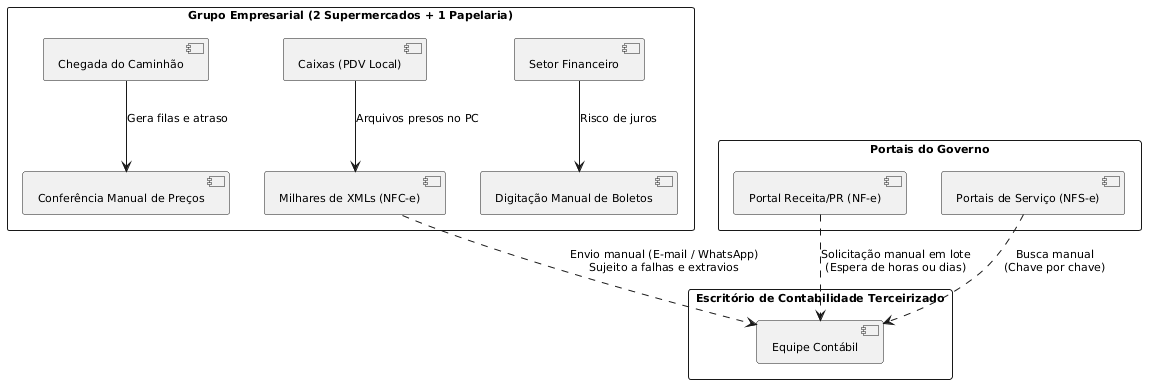
\includegraphics[width=0.9\textwidth]{problema.png}
\vspace{0.2cm}
\centerline{\footnotesize Fonte: Elaborado pelo autor (2026).}
\label{fig:problema}
\end{figure}

\subsection{Estratégia de Planejamento e Concepção Arquitetural}

Uma vez identificados os problemas operacionais e a fragmentação dos arquivos fiscais, a fase seguinte consistiu em planejar a solução tecnológica antes da codificação. Como o projeto foi conduzido por um único desenvolvedor, as metodologias ágeis foram adaptadas para o escopo individual, visando manter a organização e a previsibilidade das entregas.

O ciclo de desenvolvimento foi estruturado com base em princípios do \textit{Scrum} e do \textit{Kanban}. O projeto foi dividido em ciclos curtos de trabalho (\textit{Sprints}) orientados por módulos funcionais. Para o gerenciamento visual do fluxo de tarefas (do planejamento à conclusão), utilizou-se a ferramenta de organização Kanban, estruturando o quadro nas colunas clássicas: \textit{Backlog} (tarefas a fazer), \textit{Doing} (em desenvolvimento), \textit{Testing} (em validação) e \textit{Done} (concluído).

Para garantir que a solução atendesse simultaneamente às necessidades dos escritórios de contabilidade e dos gestores internos das empresas, a etapa de prototipação visual antecedeu a programação da interface. Utilizando ferramentas de \textit{design} de interface (como o Figma e mapeamentos no Miro), foram criados os primeiros esboços (\textit{wireframes}) das telas do painel. O objetivo dessa prototipação foi validar a disposição das informações, como os filtros de notas fiscais, a organização do módulo de contas a pagar e os botões de \textit{download} em lote,  garantindo uma Interação Humano-Computador (IHC) intuitiva para usuários sem formação técnica avançada. A Figura \ref{fig:kanban} ilustra o quadro de gestão visual utilizado para mapear as atividades do sistema e a Figura \ref{fig:tela} ilustra o mapa geral da ferramenta Figma, utilizada para prototipagem.

\begin{figure}[H]
\centering
\caption{Visão Geral - Metodologias Ágeis Utilizadas }
\vspace{0.2cm}
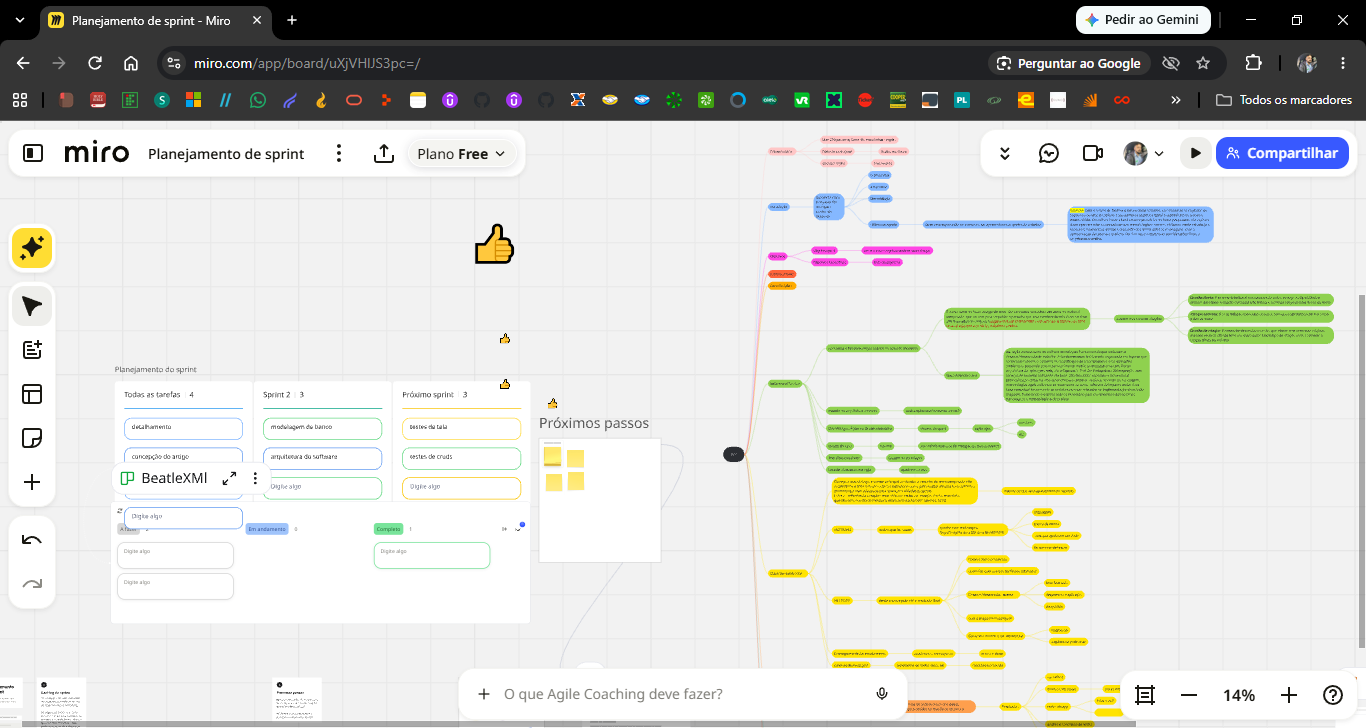
\includegraphics[width=0.9\textwidth]{kanban.png}
\vspace{0.2cm}
\centerline{\footnotesize Fonte: Elaborado pelo autor (2026).}
\label{fig:kanban}
\end{figure}

\begin{figure}[H]
\centering
\caption{Visão Geral - Prototipagem de Telas }
\vspace{0.2cm}
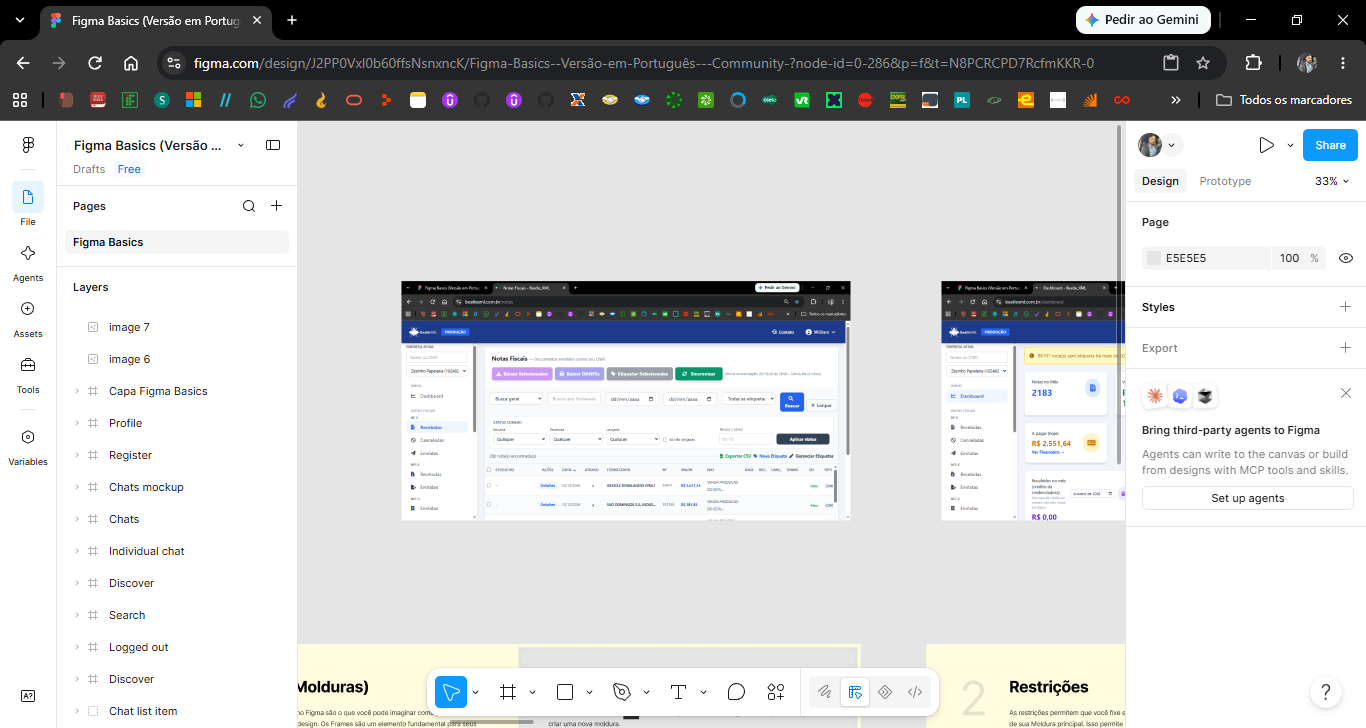
\includegraphics[width=0.9\textwidth]{tela.png}
\vspace{0.2cm}
\centerline{\footnotesize Fonte: Elaborado pelo autor (2026).}
\label{fig:tela}
\end{figure}

\subsubsection{Estudo de Viabilidade e a Documentação da SEFAZ \textit{(Secretaria de Estado da Fazenda)}}

Paralelamente ao desenho das interfaces, o planejamento exigiu um estudo profundo de viabilidade técnica voltado à comunicação com os servidores governamentais. A captura autônoma de Notas Fiscais Eletrônicas (NF-e) emitidas contra as empresas depende do consumo do \textit{Web Service} denominado \texttt{NFeDistribuicaoDFe}, disponibilizado pelo Ambiente Nacional da Receita Federal em \texttt{https://www.nfe.fazenda.gov.br/portal/principal.aspx}.

O entendimento dessa integração baseou-se na leitura do Manual de Orientação do Contribuinte (MOC), documento oficial que rege os padrões técnicos do projeto NF-e. O estudo revelou que a comunicação governamental não utiliza padrões modernos baseados em arquitetura REST e JSON (\textit{JavaScript Object Notation}), mas sim o protocolo SOAP (\textit{Simple Object Access Protocol}) versão 1.2, exigindo a montagem estrita de envelopes XML \textit{(Extensible Markup Language)} para cada requisição.

Além da formatação dos envelopes, a documentação técnica exigia que toda requisição fosse autenticada nativamente pelo protocolo \textit{Mutual TLS} (mTLS), utilizando o certificado digital e-CNPJ modelo A1 (uma certificação digital que comprova a identidade perante a Receita Federal), da empresa requerente para assinar a conexão. Antes de codificar essas regras complexas na aplicação final, realizaram-se testes isolados de requisição (utilizando ferramentas de teste de APIs \textit{(Application Programming Interfaces)}) para validar a resposta do servidor do governo, compreender o formato de compactação dos arquivos de retorno e mapear os códigos de erro, especialmente a regra temporal de "Consumo Indevido" (uma penalidade que a Receita Federal implica as novas requisições, caso não sejam seguidas as regras da API \textit{(Application Programming Interfaces)}). 

A consolidação dessas regras de negócio externas forneceu a base arquitetural para a escolha das bibliotecas de criptografia e processamento que foram adotadas na fase de codificação do \textit{backend}.


\subsection{Engenharia de Requisitos}

A partir do mapeamento dos problemas na rotina contábil e corporativa, foram definidos os requisitos do sistema visando facilitar a interação humano-computador. O Quadro \ref{qua:req_funcionais} apresenta os requisitos funcionais que delimitam as ações entregues ao usuário, enquanto o Quadro \ref{qua:req_nao_funcionais} consolida as premissas não funcionais voltadas à infraestrutura, segurança e governança.

\begin{quadro}[H]
\centering
\footnotesize
\caption{Requisitos Funcionais do Sistema BeatleXML}
\vspace{0.2cm}
\resizebox{\textwidth}{!}{%
\begin{tabular}{p{1.5cm} p{12cm}}
\toprule
\textbf{ID} & \textbf{Descrição do Requisito} \\ 
\midrule
\textbf{RF01} & O sistema deve fornecer um painel contábil que permita a visualização, configuração e o download ágil de notas fiscais em lote (arquivos ZIP separados e organizados) de todas as empresas clientes vinculadas ao perfil da empresa e do contador. \\ 
\textbf{RF02} & O sistema deve incorporar um módulo financeiro alimentado automaticamente pela leitura dos arquivos XML \textit{(Extensible Markup Language)}, podendo ser identificada pendencias, fornecedores e datas de vencimento. \\ 
\textbf{RF03} & O sistema deve permitir que o administrador do cadastro (\textit{master}) convide ativamente novos usuários (contadores, auxiliares) determinando seus níveis hierárquicos de acesso (RBAC). \\ 
\textbf{RF04} & O sistema deve disponibilizar o agente local para a empresa, denominado \textit{Beatle Uploader} para monitorar automaticamente as pastas físicas do ERP \textit{(Enterprise Resource Planning)} do cliente e transmitir silenciosamente os cupons fiscais eletrônicos (NFC-e) para a nuvem. \\ 
\textbf{RF05} & O sistema deve garantir visualização amigável de documentos no navegador, gerando Documentos Auxiliares (DANFEs) em formato PDF \textit{(Portable Document Format)} sob demanda, além de permitir o gerenciamento visual via etiquetas personalizadas. \\ 
\bottomrule
\end{tabular}%
}
\vspace{0.05cm}
\centerline{\footnotesize Fonte: Elaborado pelo autor (2026).}
\label{qua:req_funcionais}
\end{quadro}

\begin{quadro}[H]
\centering
\footnotesize
\caption{Requisitos Não Funcionais e Atributos de Segurança}
\vspace{0.2cm}
\resizebox{\textwidth}{!}{%
\begin{tabular}{p{2.5cm} p{1.5cm} p{9.5cm}}
\toprule
\textbf{Categoria} & \textbf{ID} & \textbf{Descrição e Restrição Arquitetural} \\ 
\midrule
\textbf{Segurança e Privacidade} & \textbf{RNF01} & Em conformidade com a LGPD, o sistema deve obrigar o uso de senhas fortes com criptografia (\textit{bcrypt}), proteger telas de entrada com reCAPTCHA e oferecer Verificação em Dois Fatores (2FA) via e-mail. \\ 
\textbf{Isolamento Multi-tenant} & \textbf{RNF02} & O acesso aos dados deve ser validado dinamicamente na camada de aplicação através de \textit{tokens} JWT \textit{(JSON Web Token)}, assegurando que um contador não visualize as notas de empresas pelas quais não possui autorização. \\ 
\textbf{Confiabilidade de Rede} & \textbf{RNF03} & A integração com a SEFAZ \textit{(Secretaria de Estado da Fazenda)} deve implementar \textit{workers} assíncronos capazes de aplicar mecanismos para seguir rigidamente as regras impostas no documento oficial da API \textit{(Application Programming Interfaces)} da Receita Federal. \\ 
\bottomrule
\end{tabular}%
}
\vspace{0.05cm}
\centerline{\footnotesize Fonte: Elaborado pelo autor (2026).}
\label{qua:req_nao_funcionais}
\end{quadro}

\subsection{Arquitetura do Sistema e Stack Tecnológica}
% Aqui voce vai contar tudo sobre as tecnologias e o motivo que eu escolhi cada uma, mostrar a estrutura do projeto (onde estão as rotas, roles e principais) e sua arquitetura, falar sobre backend e por que o "front" é interligado, pode ser acrescentado mais sessões como 3.4.1 e etc. Ou seja, Aqui voce vai explicar ao orientador as tecnologias e motivos de serem escolhidas.
\subsection{Modelagem de Dados e Persistência}
% Aqui voce vai explicar o banco de dados e sua estrutura, suas principais tabelas, a segurança das senhas, as tecnologias, como a lgpd é implantada aqui, os "roles", as relações principais e etc.
\subsection{Segurança da Informação e Conformidade (LGPD)}
\subsection{Concorrência e Regras de Negócio}
% O que vamos contar: O coração da confiança do seu sistema. Mostraremos como o sistema isola as empresas (\textit{Tenant Isolation}) através de tokens JWT, como as senhas são protegidas com \textit{bcrypt}, e a grande sacada: como o Certificado A1 do cliente não fica "jogado" em uma pasta, mas sim criptografado no banco de dados com a biblioteca \textit{Fernet}. pode-se explicar que a internet do governo é lenta e, por isso, usamos processos em segundo plano (\textit{background workers}) e como eles funcionam. Como o sistema segue as regras da receita, aplica um bloqueio preventivo de 2 horas na base de dados, salvando o IP do servidor de banimentos e permitindo que o contador continue trabalhando
\subsection{Automação Local: O Agente Beatle Uploader}
% O que vamos contar: Para fechar a metodologia, explicaremos como resolvemos o problema das notas de balcão (NFC-e). Explicaremos o uso da biblioteca \textit{watchdog} (escuta do sistema operacional) para capturar os XMLs gerados pelo ERP da loja e enviá-los silenciosamente para a nuvem.


% ================= RESULTADOS E DISCUSSÕES =================
\section{Resultados e Discussões}

em andamento ...
...
..

% ================= CONCLUSÃO =================
\section{Considerações Finais}
em andamento...
..
..

\section*{Declarações}

\textbf{Uso de Inteligência Artificial:} Durante a preparação deste trabalho, o(s) autor(es) utilizou(aram) o Google Gemini com o objetivo de aprimorar a redação, organizar o contexto de requisitos e revisar a linguagem acadêmica. Após o uso da ferramenta, o(s) autor(es) executou(aram) a revisão final, garantindo o alinhamento com o código-fonte original, assumindo total responsabilidade pela integridade técnica da publicação.

\textbf{Financiamento:} Os autores declaram que nenhum suporte financeiro de agências públicas ou privadas foi recebido durante o desenvolvimento deste manuscrito.

\textbf{Conflito de Interesses:} Os autores declaram não possuir interesses financeiros concorrentes que pudessem influenciar as decisões metodológicas expostas neste artigo.

\textbf{Disponibilidade de Dados:} Os diagramas de fluxo, a estrutura relacional e o código-fonte gerencial detalhados nesta pesquisa encontram-se registrados e estão publicamente acessíveis através do repositório oficial: \url{https://github.com/Willfragatta/TCC-BeatleXml.git}.

\bibliographystyle{sbc}
\bibliography{referencias}

\end{document}